\chapter{Specifikacija programske potpore}
		
	\section{Funkcionalni zahtjevi}
			
			\textbf{\textit{dio 1. revizije}}\\
			
			\textit{Navesti \textbf{dionike} koji imaju \textbf{interes u ovom sustavu} ili  \textbf{su nositelji odgovornosti}. To su prije svega korisnici, ali i administratori sustava, naručitelji, razvojni tim.}\\
				
			\textit{Navesti \textbf{aktore} koji izravno \textbf{koriste} ili \textbf{komuniciraju sa sustavom}. Oni mogu imati inicijatorsku ulogu, tj. započinju određene procese u sustavu ili samo sudioničku ulogu, tj. obavljaju određeni posao. Za svakog aktora navesti funkcionalne zahtjeve koji se na njega odnose.}\\
			
			
			\noindent \textbf{Dionici:}
			
			\begin{packed_enum}
				
				\item Naručitelj
				\item Korisnici
				\begin{enumerate}
					\item Voditelji
					\item Istraživači
					\item  Tragači
				\end{enumerate}		
				\item Administrator
				\item Razvojni tim 
				
			\end{packed_enum}
			
			\noindent \textbf{Aktori i njihovi funkcionalni zahtjevi:}
			
			
			\begin{packed_enum}
				\item  \underbar{Neregistrirani korisnik (inicijator) može:}
				
				\begin{packed_enum}
					
					\item može poslati zahtjev za registraciju s željenom ulogom za koju se prijavljuje
					
				\end{packed_enum}
			
				\item  \underbar{Voditelj postaje (inicijator) može:}
				
				\begin{packed_enum}
					
					\item definira koji su tragači dio njegove postaje 
					\item definira na koji način su osposobljeni izvoditi pretraživanje 
					\item odabire konkretne tragače koji će sudjelovati u akciji 
					
				\end{packed_enum}
				
				\item  \underbar{Istraživač (inicijator) može:}
				
				\begin{packed_enum}
					
					\item može bilježiti i vizualizirati staze kojima su tragači putovali i način kojim su se kretali u obliku toplinskih karata 
					\item mogu stvoriti nove akcije pretraživanja i praćenja s detaljima o određenim vrstama, jedinkama ili staništima za proučavanje 
					\item može poslati zahtjev za tragačima s opisom o potrebnim kvalifikacijama voditelju postaje 
					\item preko karte tragačima pojedinačno zadaje zadatke 
					\item informacije o pozicijama životinja, tragača i postaja mu se pokazuju preko interaktivne karte
					\begin{packed_enum}
					
						\item  može odabrati da se za izradu karata koriste neka od idućih informacija: povijesne pozicije svih praćenih životinja, filtrirano po vrsti ili pojedinačno po jedinki te trenutne pozicije praćenih životinja 
					
					\end{packed_enum}
					\item može ostaviti komentar za ostale sudionike u akciji 
					\item može ostaviti komentar za svaki zadatak 
					
				\end{packed_enum}
				
				\item  \underbar{Tragač (inicijator) može:}
				
				\begin{packed_enum}
					
					\item može biti osposobljen za obavljanje zadataka pješke, dronom, automobilom, cross motorom, brodom ili helikopterom 
					\item može praćenoj životinji tijekom akcije ostaviti komentar 
					\item može se maknuti s akcije završetkom svih potrebnih zadataka 
					\item na karti mu se prikazuju zadaci koje treba obaviti, trenutna pozicija ostalih tragača aktivnih na istoj akciji, te trenutna pozicija praćenih životinja 
					\item može ostaviti komentar za ostale sudionike u akciji 
					
				\end{packed_enum}
				
				\item  \underbar{Administrator (inicijator) može:}
				
				\begin{packed_enum}
					
					\item može vidjeti popis svih registriranih korisnika i njihovih osobnih podataka  
					\item može svim registriranim korisnicima mijenjati dodijeljena prava i osobne podatke 
					\item dodatno potvrđuje istraživača i voditelja postaje tijekom prijave 
					
				\end{packed_enum}
				
				\item  \underbar{Baza podataka (sudionik): može:}
				
				\begin{packed_enum}
					
					\item pohranjuje sve podatke o korisnicima i njihovim ovlastima 
					\item pohranjuje sve podatke o akcijama, lokacijama, životinjama i sl. 
					
				\end{packed_enum}
			\end{packed_enum}
			
			\eject 
			
			
				
			\subsection{Obrasci uporabe}
				
				\textbf{\textit{dio 1. revizije}}
				
				\subsubsection{Opis obrazaca uporabe}
					\textit{Funkcionalne zahtjeve razraditi u obliku obrazaca uporabe. Svaki obrazac je potrebno razraditi prema donjem predlošku. Ukoliko u nekom koraku može doći do odstupanja, potrebno je to odstupanje opisati i po mogućnosti ponuditi rješenje kojim bi se tijek obrasca vratio na osnovni tijek.}\\
					

					\noindent \underbar{\textbf{UC1 -Registracija}}
					\begin{packed_item}
	
						\item \textbf{Glavni sudionik: }Neregistrirani korisnik
						\item  \textbf{Cilj:} Stvoriti korisnički račun za pristup sustavu
						\item  \textbf{Sudionici:} Baza podataka
						\item  \textbf{Preduvjet:} -
						\item  \textbf{Opis osnovnog tijeka:}
						
						\item[] \begin{packed_enum}
	
							\item Korisnik odabire opciju za registraciju  
							\item Korisnik unosi potrebne korisničke podatke (korisničko ime, fotografija, lozinka, ime, prezime i email adresa) te odabire željenu ulogu za koju se prijavljuje 
							\item Korisnik prima obavijest o uspješnoj/neuspješnoj registraciji
						\end{packed_enum}
						
						\item  \textbf{Opis mogućih odstupanja:}
						
						\item[] \begin{packed_item}
	
							\item[2.a] Odabir već zauzetog korisničkog imena i/ili e-maila, unos korisničkog podatka u nedozvoljenom formatu ili pružanje neispravnoga e-maila 
							\item[] \begin{packed_enum}
								
								\item Sustav obavještava korisnika o neuspjelom upisu i vraća ga na stranicu za registraciju 
								\item Korisnik mijenja potrebne podatke te završava unos ili odustaje od registracije 
								
							\end{packed_enum}
							\item[3.a] Administrator odbija registraciju korisnika koji se želi registrirati kao istraživač ili voditelj
							\item[] \begin{packed_enum}
								
								\item Sustav obavještava korisnika o neuspjelom upisu i vraća ga na stranicu za registraciju 
								
							\end{packed_enum}
							
						\end{packed_item}
					\end{packed_item}
				
					\noindent \underbar{\textbf{UC2 -Potvrda registracije}}
					\begin{packed_item}
						
						\item \textbf{Glavni sudionik: }Administrator
						\item  \textbf{Cilj:} Potvrditi/odbiti registraciju korisnika koji se želi registrirati kao istraživač/voditelj 
						\item  \textbf{Sudionici:} Baza podataka, neregistrirani korisnik 
						\item  \textbf{Preduvjet:} Korisnik je poslao zahtjev za registraciju kao istraživač/voditelj 
						\item  \textbf{Opis osnovnog tijeka:}
						
						\item[] \begin{packed_enum}
							
							\item Administrator odabire opciju pregleda zahtjeva 
							\item Administrator odabire zahtjev 
							\item Administrator  odabire opciju potvrdi/odbij 
							\item Ako administrator potvrdi, sustav ažurira bazu podataka s novim korisnikom
						\end{packed_enum}
					\end{packed_item}
					
					\noindent \underbar{\textbf{UC3 -Pregled svih korisnika}}
					\begin{packed_item}
						
						\item \textbf{Glavni sudionik: }Administrator
						\item  \textbf{Cilj:} Pregledati sve registrirane korisnike i njihove osobne podatke
						\item  \textbf{Sudionici:} Baza podataka
						\item  \textbf{Preduvjet:} -
						\item  \textbf{Opis osnovnog tijeka:}
						
						\item[] \begin{packed_enum}
							
							\item Administrator odabire opciju pregled korisnika 
							\item Aplikacija prikazuje sve registrirane korisnike i njihove osobne podatke
						\end{packed_enum}
					\end{packed_item}
					
					\noindent \underbar{\textbf{UC4 -Mijenjanje podataka korisnika}}
					\begin{packed_item}
						
						\item \textbf{Glavni sudionik: }Administrator
						\item  \textbf{Cilj:} Promijeniti dodijeljena prava i osobne podatke korisnika 
						\item  \textbf{Sudionici:} Baza podataka
						\item  \textbf{Preduvjet:} Postoji barem jedan registrirani korisnik
						\item  \textbf{Opis osnovnog tijeka:}
						
						\item[] \begin{packed_enum}
							
							\item Administrator odabire opciju za promjenu podataka 
							\item Administrator radi promjene 
							\item Administrator sprema promjene 
							\item Sustav ažurira bazu podataka
						\end{packed_enum}
						
						\item  \textbf{Opis mogućih odstupanja:}
						
						\item[] \begin{packed_item}
							
							\item[3.a] Administrator promijeni podatke, ali ne odabere opciju ”Spremi promjenu” 
							\item[] \begin{packed_enum}
								
								\item Sustav obavještava administratora da nije spremio podatke prije izlaska iz prozora
								
							\end{packed_enum}
							
						\end{packed_item}
					\end{packed_item}
					
					\noindent \underbar{\textbf{UC5 -Prijava u sustav}}
					\begin{packed_item}
						
						\item \textbf{Glavni sudionik: }Korisnik
						\item  \textbf{Cilj:} Pristup korisničkom sučelju 
						\item  \textbf{Sudionici:} Baza podataka
						\item  \textbf{Preduvjet:} Korisnik ima registrirani korisnički račun
						\item  \textbf{Opis osnovnog tijeka:}
						
						\item[] \begin{packed_enum}
							
							\item Unos korisničkog imena i lozinke 
							\item Potvrda o ispravnosti unesenih podataka 
							\item Pristup korisničkim funkcijama
						\end{packed_enum}
						
						\item  \textbf{Opis mogućih odstupanja:}
						
						\item[] \begin{packed_item}
							
							\item[1.a] Neispravno korisničko ime/lozinka
							\item[] \begin{packed_enum}
								
								\item Sustav obavještava korisnika o neuspjelom upisu i vraća ga na stranicu za registraciju 
								
							\end{packed_enum}
							
						\end{packed_item}
					\end{packed_item}
					
					\noindent \underbar{\textbf{UC6 -Definiranje tragača za postaju}}
					\begin{packed_item}
						
						\item \textbf{Glavni sudionik: }Voditelj postaje
						\item  \textbf{Cilj:} Definirati koji tragači pripadaju postaji koju vodi određeni voditelj 
						\item  \textbf{Sudionici:} Baza podataka
						\item  \textbf{Preduvjet:} Voditelj je prijavljen i postoji slobodnih tragača za postaju
						\item  \textbf{Opis osnovnog tijeka:}
						
						\item[] \begin{packed_enum}
							
							\item Voditelj postaje bira opciju "Definiraj tragače za postaju" 
							\item Sustav prikazuje popis slobodnih tragača koji nisu dodijeljeni nijednoj postaji 
							\item Voditelj odabire tragače koje želi dodijeliti svojoj postaji 
							\item Voditelj potvrđuje odabir 
							\item Sustav ažurira bazu podataka i dodjeljuje odabrane tragače postaji koju vodi voditelj 
						\end{packed_enum}
					\end{packed_item}
					
					\noindent \underbar{\textbf{UC7 - Definiranje načina izvođenja pretraživanja}}
					\begin{packed_item}
						
						\item \textbf{Glavni sudionik: }Voditelj postaje
						\item  \textbf{Cilj:} Definirati na koji način su tragači osposobljeni izvoditi pretraživanje (pješke, dronom, automobilom, cross motorom, brodom ili helikopterom) 
						\item  \textbf{Sudionici:} Baza podataka
						\item  \textbf{Preduvjet:} Voditelj je prijavljen i postoje tragači koji pripadaju njegovoj postaji
						\item  \textbf{Opis osnovnog tijeka:}
						
						\item[] \begin{packed_enum}
							
							\item Voditelj postaje odabire opciju "Definiraj načine pretraživanja" 
							\item Sustav prikazuje moguće načine pretraživanja za njegovu postaju 
							\item Voditelj odabire željene načine pretraživanja 
							\item Voditelj potvrđuje odabir 
							\item Sustav ažurira bazu podataka s odabranim načinima pretraživanja 
						\end{packed_enum}
					\end{packed_item}
					
					\noindent \underbar{\textbf{UC8 -Biranje tragača za akciju}}
					\begin{packed_item}
						
						\item \textbf{Glavni sudionik: }Voditelj postaje
						\item  \textbf{Cilj:} Odabrati koji tragači će sudjelovati u nekoj akciji
						\item  \textbf{Sudionici:} Baza podataka
						\item  \textbf{Preduvjet:} Voditelj je prijavljen i postoje tragači koji pripadaju njegovoj postaji
						\item  \textbf{Opis osnovnog tijeka:}
						
						\item[] \begin{packed_enum}
							
							\item Voditelj postaje odabire opciju "Odaberi tragače za akciju" 
							\item Sustav prikazuje popis tragača koji pripadaju postaji voditelja 
							\item Voditelj odabire tragače koje želi uključiti u akciju 
							\item Voditelj potvrđuje odabir 
							\item Sustav ažurira bazu podataka i dodjeljuje odabrane tragače akciji 
						\end{packed_enum}
					\end{packed_item}
					
					\noindent \underbar{\textbf{UC9 -Ostavljanje komentara za praćenu životinju}}
					\begin{packed_item}
						
						\item \textbf{Glavni sudionik: }Tragač
						\item  \textbf{Cilj:} Ostaviti komentar praćenoj životinji
						\item  \textbf{Sudionici:} Baza podataka
						\item  \textbf{Preduvjet:} Tragač je prijavljen te je u akciji praćenja životinje
						\item  \textbf{Opis osnovnog tijeka:}
						
						\item[] \begin{packed_enum}
							
							\item Tragač odabire opciju "Ostavi komentar za životinju" 
							\item Sustav prikazuje polje za unos komentara 
							\item Tragač unosi željeni komentar 
							\item Tragač potvrđuje unos 
							\item Sustav ažurira bazu podataka s novim komentarom za praćenu životinju 
						\end{packed_enum}
					\end{packed_item}
					
					\noindent \underbar{\textbf{UC10 -Ostavljanje komentara drugim sudionicima (tragač)}}
					\begin{packed_item}
						
						\item \textbf{Glavni sudionik: }Tragač
						\item  \textbf{Cilj:} Ostaviti komentar drugim sudionicima akcije 
						\item  \textbf{Sudionici:} Baza podataka
						\item  \textbf{Preduvjet:} Tragač je prijavljen, sudjeluje u akciji i ima otvorenu kartu
						\item  \textbf{Opis osnovnog tijeka:}
						
						\item[] \begin{packed_enum}
							
							\item Tragač odabire opciju "Ostavi komentar za sudionike" 
							\item Sustav prikazuje polje za unos komentara 
							\item Tragač unosi željeni komentar 
							\item Tragač potvrđuje unos 
							\item Sustav ažurira bazu podataka s novim komentarom za sudionike akcije 
						\end{packed_enum}
					\end{packed_item}
					
					\noindent \underbar{\textbf{UC11 -Ostavljanje komentara drugim sudionicima (istraživač) }}
					\begin{packed_item}
						
						\item \textbf{Glavni sudionik: }Istraživač
						\item  \textbf{Cilj:} Ostaviti komentar praćenoj životinji 
						\item  \textbf{Sudionici:} Baza podataka
						\item  \textbf{Preduvjet:} Istraživač je prijavljen, sudjeluje u akciji i ima otvorenu kartu
						\item  \textbf{Opis osnovnog tijeka:}
						
						\item[] \begin{packed_enum}
							
							\item Istraživač odabire opciju "Ostavi komentar za sudionike" 
							\item Sustav prikazuje polje za unos komentara 
							\item Tragač unosi željeni komentar 
							\item Tragač potvrđuje unos 
							\item Sustav ažurira bazu podataka s novim komentarom za sudionike akcije 
						\end{packed_enum}
					\end{packed_item}
					
					\noindent \underbar{\textbf{UC12 -Micanje s akcije}}
					\begin{packed_item}
						
						\item \textbf{Glavni sudionik: }Tragač
						\item  \textbf{Cilj:} Maknuti se sa akcije u kojoj je završio sve svoje zadatke 
						\item  \textbf{Sudionici:} Baza podataka
						\item  \textbf{Preduvjet:} Tragač je prijavljen te je završio sve potrebne zadatke u akciji 
						\item  \textbf{Opis osnovnog tijeka:}
						
						\item[] \begin{packed_enum}
							
							\item Tragač odabire opciju "Napusti akciju" 
							\item Sustav provjerava je li tragač završio sve svoje zadatke u akciji 
							\item Ako su svi zadaci završeni, sustav tragača uklanja s akcije 
							\item Sustav ažurira bazu podataka 
						\end{packed_enum}
					\end{packed_item}
					
					\noindent \underbar{\textbf{UC13 -Pregled karte}}
					\begin{packed_item}
						
						\item \textbf{Glavni sudionik: }Tragač
						\item  \textbf{Cilj:} Pristupiti karti za pregled zadataka koje treba obaviti, trenutne pozicije ostalih tragača aktivnih na istoj akciji, te trenutne pozicije praćenih životinja
						\item  \textbf{Sudionici:} Baza podataka
						\item  \textbf{Preduvjet:} Tragač je prijavljen te sudjeluje u akciji 
						\item  \textbf{Opis osnovnog tijeka:}
						
						\item[] \begin{packed_enum}
							
							\item Tragač odabire opciju "Pregledaj kartu" 
							\item Sustav prikazuje kartu s označenim zadacima, pozicijama tragača i praćenih životinja 
							\item Tragač može interaktivno pregledavati kartu i pratiti informacije o akciji
						\end{packed_enum}
					\end{packed_item}
					
					\noindent \underbar{\textbf{UC14 -Bilježenje i vizualizacija staze}}
					\begin{packed_item}
						
						\item \textbf{Glavni sudionik: }Istraživač
						\item  \textbf{Cilj:} Zabilježiti i vizualizirati stazu radi bolje daljnje analize
						\item  \textbf{Sudionici:} Baza podataka
						\item  \textbf{Preduvjet:} Istraživač je prijavljen te postoji staza koju želi zabilježiti i/ili vizualizirati
						\item  \textbf{Opis osnovnog tijeka:}
						
						\item[] \begin{packed_enum}
							
							\item Istraživač odabire opciju "Bilježenje staze" 
							\item Sustav započinje snimanje staze i bilježi koordinate 
							\item Istraživač završava snimanje staze 
							\item Sustav prikazuje vizualizaciju snimljene staze
						\end{packed_enum}
					\end{packed_item}
					
					\noindent \underbar{\textbf{UC15 -Stvaranje novih akcija}}
					\begin{packed_item}
						
						\item \textbf{Glavni sudionik: }Istraživač
						\item  \textbf{Cilj:} Stvoriti novu akciju pretraživanja i praćenja s detaljima o određenim vrstama, jedinkama ili staništima za proučavanje 
						\item  \textbf{Sudionici:} Baza podataka
						\item  \textbf{Preduvjet:} Istraživač je prijavljen te postoje slobodni tragači kod određene postaje
						\item  \textbf{Opis osnovnog tijeka:}
						
						\item[] \begin{packed_enum}
							
							\item Istraživač odabire opciju "Stvori novu akciju" 
							\item Sustav prikazuje obrazac za unos detalja o akciji 
							\item Istraživač unosi željene podatke 
							\item Istraživač potvrđuje unos 
							\item Sustav ažurira bazu podataka s novom akcijom 
						\end{packed_enum}
					\end{packed_item}
					
					\noindent \underbar{\textbf{UC16 -Slanje zahtjeva za tragačima}}
					\begin{packed_item}
						
						\item \textbf{Glavni sudionik: }Istraživač
						\item  \textbf{Cilj:} Voditelju postaje poslati zahtjev za tragačima s opisom o potrebnim kvalifikacijama
						\item  \textbf{Sudionici:} Baza podataka, voditelj postaje
						\item  \textbf{Preduvjet:} Istraživač je prijavljen i postoji barem jedan voditelj postaje s tragačima u svojoj postaji 
						\item  \textbf{Opis osnovnog tijeka:}
						
						\item[] \begin{packed_enum}
							
							\item Istraživač odabire opciju "Pošalji zahtjev za tragačima" 
							\item Sustav prikazuje obrazac za unos detalja o zahtjevu (kvalifikacije, broj tragača, itd.) 
							\item Istraživač unosi željene podatke 
							\item Istraživač šalje zahtjev voditelju postaje 
							\item Voditelj postaje prima zahtjev i može ga prihvatiti ili odbiti 
							\item Ako voditelj prihvati, sustav ažurira bazu podataka s novim tragačima za akciju 
						\end{packed_enum}
					\end{packed_item}
					
					\noindent \underbar{\textbf{UC17 -Dodjela zadatka tragaču}}
					\begin{packed_item}
						
						\item \textbf{Glavni sudionik: }Istraživač
						\item  \textbf{Cilj:} Određen zadatak akcije dodijeliti nekom tragaču u toj istoj akciji 
						\item  \textbf{Sudionici:} Baza podataka, tragač
						\item  \textbf{Preduvjet:} Istraživač je prijavljen te sudjeluje u nekoj akciji u kojoj sudjeluje barem jedan tragač 
						\item  \textbf{Opis osnovnog tijeka:}
						
						\item[] \begin{packed_enum}
							
							\item Istraživač odabire opciju "Dodijeli zadatak tragaču" 
							\item Sustav prikazuje popis tragača koji sudjeluju u istoj akciji 
							\item Istraživač odabire tragača kojem želi dodijeliti zadatak
							\item Istraživač odabire specifični zadatak koji želi dodijeliti tragaču 
							\item Istraživač potvrđuje dodjelu zadatka 
							\item Sustav ažurira bazu podataka s dodijeljenim zadatkom tragaču 
						\end{packed_enum}
					\end{packed_item}
					
					\noindent \underbar{\textbf{UC18 -Stvaranje interaktivne karte}}
					\begin{packed_item}
						
						\item \textbf{Glavni sudionik: }Istraživač
						\item  \textbf{Cilj:} Stvoriti interaktivnu kartu 
						\item  \textbf{Sudionici:} Baza podataka
						\item  \textbf{Preduvjet:} Istraživač je prijavljen
						\item  \textbf{Opis osnovnog tijeka:}
						
						\item[] \begin{packed_enum}
							
							\item Istraživač odabire opciju "Stvori interaktivnu kartu" 
							\item Sustav prikazuje alate za izradu interaktivne karte  
							\item Istraživač uređuje kartu prema svojim potrebama 
							\item Istraživač potvrđuje stvaranje karte 
							\item Sustav pohranjuje interaktivnu kartu u bazu podataka 
						\end{packed_enum}
					\end{packed_item}
					
					\noindent \underbar{\textbf{UC19 -Ostavljanje komentara za zadatak}}
					\begin{packed_item}
						
						\item \textbf{Glavni sudionik: }Istraživač
						\item  \textbf{Cilj:} Ostaviti tragaču/tragačima komentar za neki zadatak 
						\item  \textbf{Sudionici:} Baza podataka
						\item  \textbf{Preduvjet:} Istraživač je prijavljen te sudjeluje u akciji 
						\item  \textbf{Opis osnovnog tijeka:}
						
						\item[] \begin{packed_enum}
							
							\item Istraživač odabire opciju "Ostavi komentar za zadatak" 
							\item Sustav prikazuje popis zadataka dostupnih za komentiranje 
							\item Istraživač odabire zadatak kojem želi ostaviti komentar 
							\item Istraživač unosi željeni komentar 
							\item Istraživač potvrđuje unos 
							\item Sustav ažurira bazu podataka s novim komentarom za zadatak 
						\end{packed_enum}
					\end{packed_item}
					
				\subsubsection{Dijagrami obrazaca uporabe}
					\begin{figure}[H]
						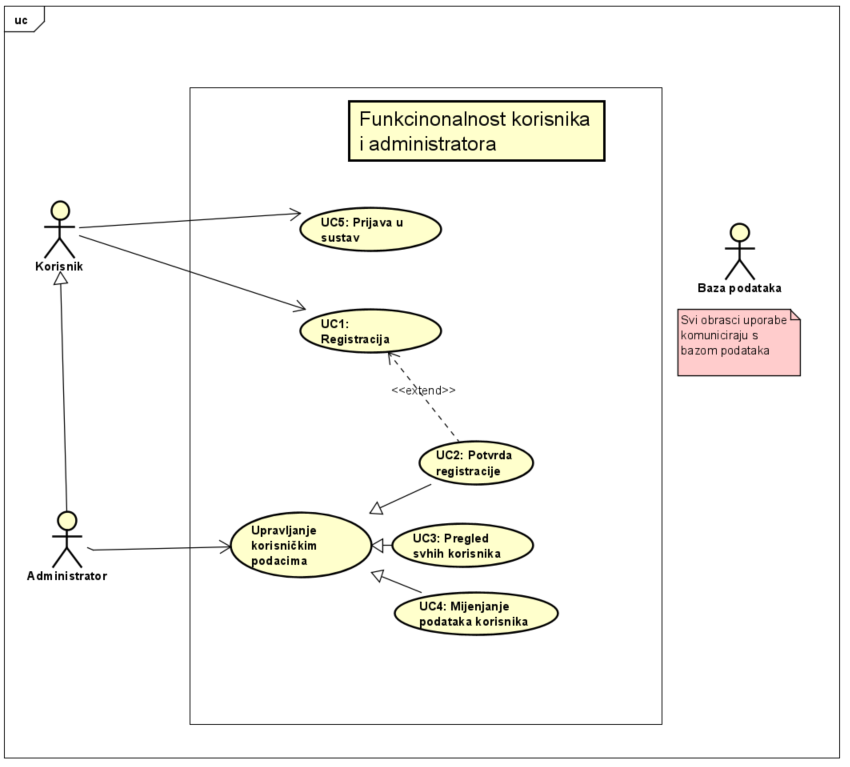
\includegraphics[scale=0.8]{dijagrami/Korisnik-admin-dijagram.PNG} 
						\centering
						\caption{Dijagram obrasca uporabe, funkcionalnost korisnika i administratora}
						\label{fig:promjene}
					\end{figure}	
					
					\begin{figure}[H]
						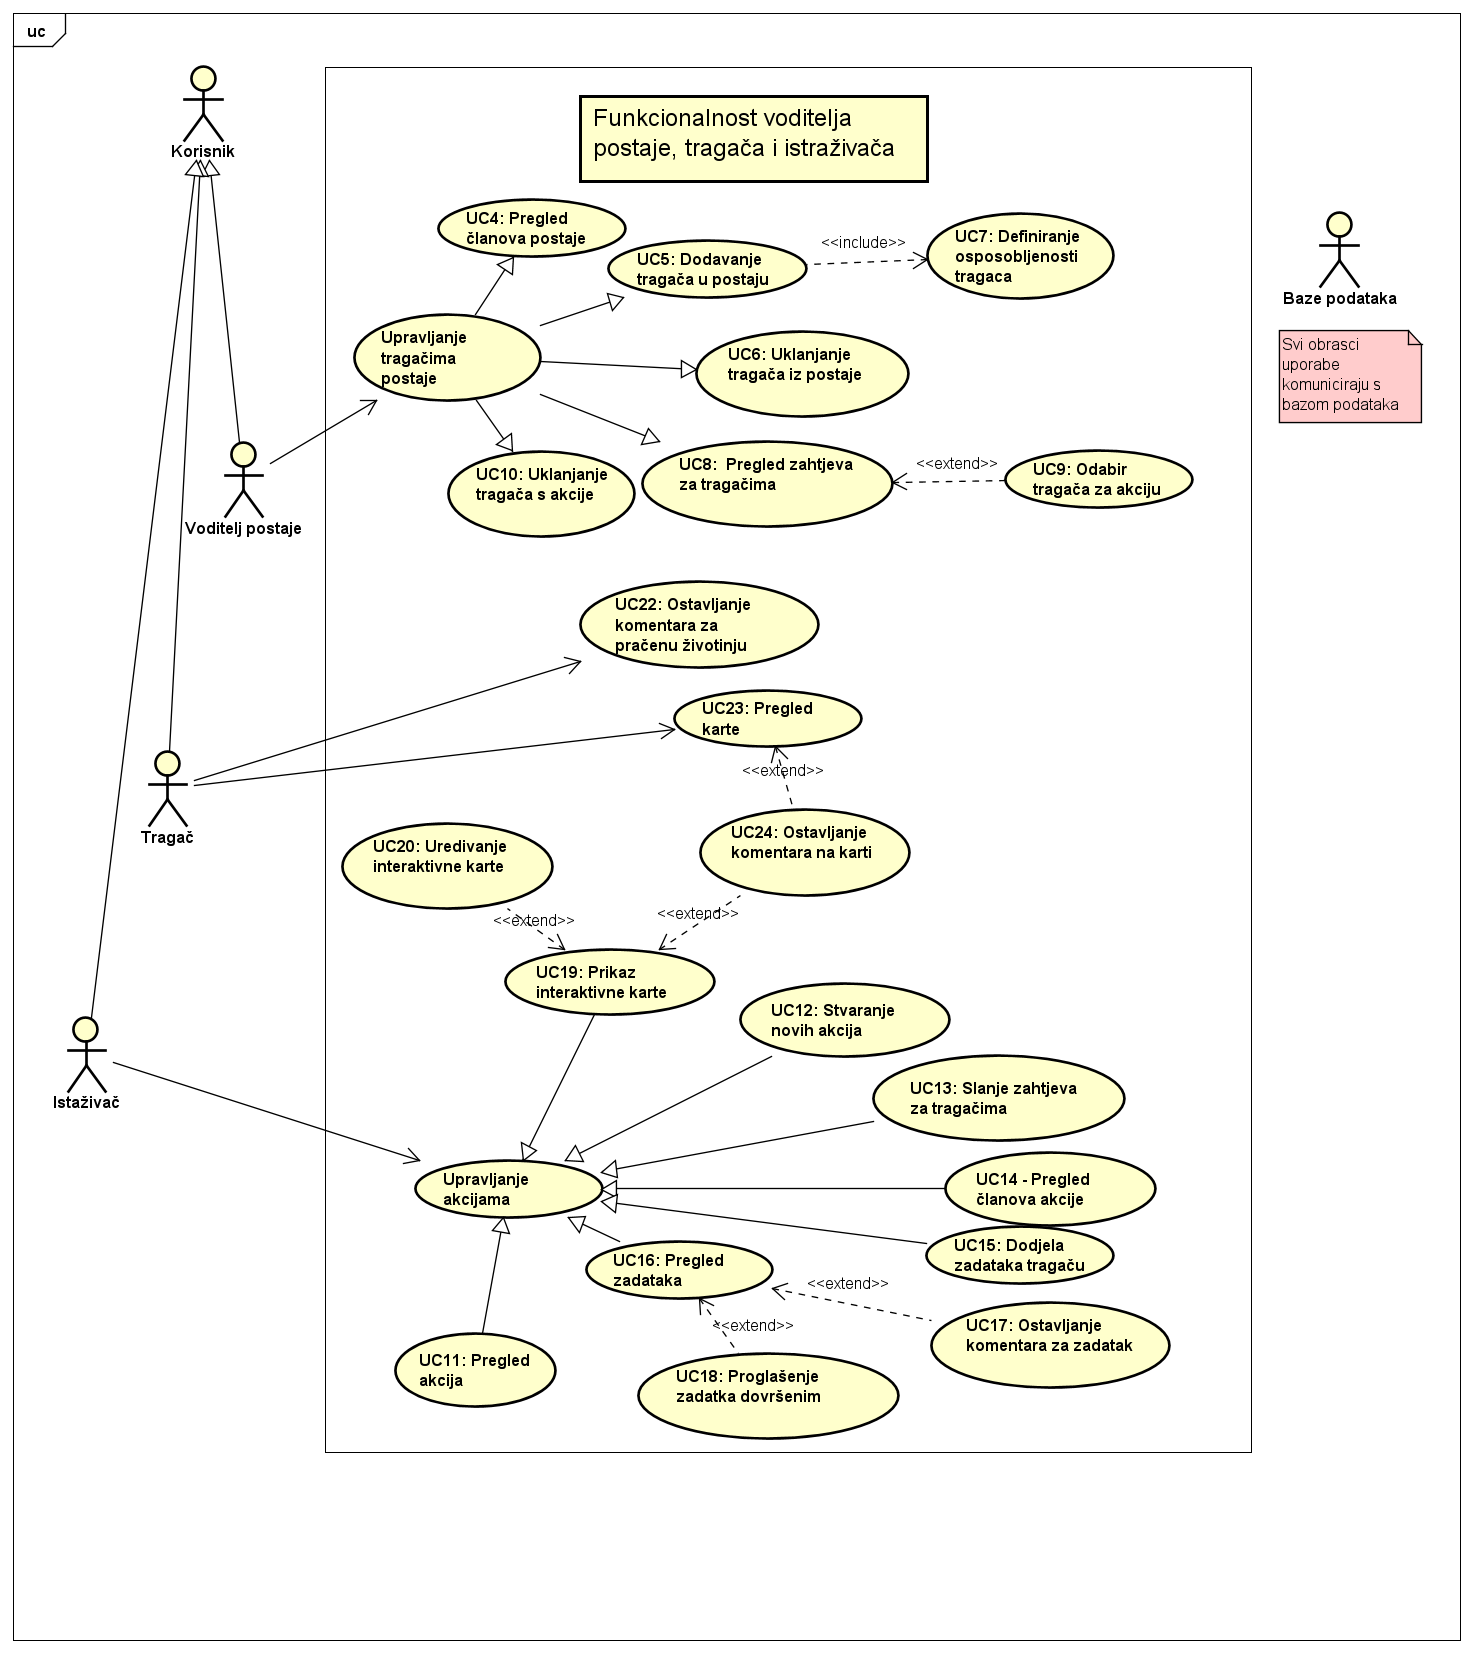
\includegraphics[scale=1]{dijagrami/voditelj-tragac-istrazivac-dijagram.PNG} 
						\centering
						\caption{Dijagram obrasca uporabe, voditelja postaje, tragača i istraživača}
						\label{fig:promjene}
					\end{figure}	
				
				
			\subsection{Sekvencijski dijagrami}
				
				\textbf{\textit{dio 1. revizije}}\\
				
				\textit{Nacrtati sekvencijske dijagrame koji modeliraju najvažnije dijelove sustava (max. 4 dijagrama). Ukoliko postoji nedoumica oko odabira, razjasniti s asistentom. Uz svaki dijagram napisati detaljni opis dijagrama.}
				\eject
	
		\section{Ostali zahtjevi}
		
			\textbf{\textit{dio 1. revizije}}\\
		 
			 \textit{Nefunkcionalni zahtjevi i zahtjevi domene primjene dopunjuju funkcionalne zahtjeve. Oni opisuju \textbf{kako se sustav treba ponašati} i koja \textbf{ograničenja} treba poštivati (performanse, korisničko iskustvo, pouzdanost, standardi kvalitete, sigurnost...). Primjeri takvih zahtjeva u Vašem projektu mogu biti: podržani jezici korisničkog sučelja, vrijeme odziva, najveći mogući podržani broj korisnika, podržane web/mobilne platforme, razina zaštite (protokoli komunikacije, kriptiranje...)... Svaki takav zahtjev potrebno je navesti u jednoj ili dvije rečenice.}
			 
			 
			 
	